\documentclass[journal]{vgtc}                % final (journal style)
%\documentclass[review,journal]{vgtc}         % review (journal style)
%\documentclass[widereview]{vgtc}             % wide-spaced review
%\documentclass[preprint,journal]{vgtc}       % preprint (journal style)

% Colors
\usepackage[
hyperref,% for working together with hyperref
table% for coloring matrix entries
]{xcolor}% color package; load before tocstyle

%% Uncomment one of the lines above depending on where your paper is
%% in the conference process. ``review'' and ``widereview'' are for review
%% submission, ``preprint'' is for pre-publication, and the final version
%% doesn't use a specific qualifier.

%% Please use one of the ``review'' options in combination with the
%% assigned online id (see below) ONLY if your paper uses a double blind
%% review process. Some conferences, like IEEE Vis and InfoVis, have NOT
%% in the past.

%% Please note that the use of figures other than the optional teaser is not permitted on the first page
%% of the journal version.  Figures should begin on the second page and be
%% in CMYK or Grey scale format, otherwise, colour shifting may occur
%% during the printing process.  Papers submitted with figures other than the optional teaser on the
%% first page will be refused. Also, the teaser figure should only have the
%% width of the abstract as the template enforces it.

%% These few lines make a distinction between latex and pdflatex calls and they
%% bring in essential packages for graphics and font handling.
%% Note that due to the \DeclareGraphicsExtensions{} call it is no longer necessary
%% to provide the the path and extension of a graphics file:
%% 
\includegraphics{diamondrule} is completely sufficient.
%%
\ifpdf%                                % if we use pdflatex
  \pdfoutput=1\relax                   % create PDFs from pdfLaTeX
  \pdfcompresslevel=9                  % PDF Compression
  \pdfoptionpdfminorversion=7          % create PDF 1.7
  \ExecuteOptions{pdftex}
  \usepackage{graphicx}                % allow us to embed graphics files
  \DeclareGraphicsExtensions{.pdf,.png,.jpg,.jpeg} % for pdflatex we expect .pdf, .png, or .jpg files
\else%                                 % else we use pure latex
  \ExecuteOptions{dvips}
  \usepackage{graphicx}                % allow us to embed graphics files
  \DeclareGraphicsExtensions{.eps}     % for pure latex we expect eps files
\fi%

%% it is recomended to use ``\autoref{sec:bla}'' instead of ``Fig.~\ref{sec:bla}''
\graphicspath{{figures/}{pictures/}{images/}{./}} % where to search for the images

\usepackage{microtype}                 % use micro-typography (slightly more compact, better to read)
\PassOptionsToPackage{warn}{textcomp}  % to address font issues with \textrightarrow
\usepackage{textcomp}                  % use better special symbols
\usepackage{mathptmx}                  % use matching math font
\usepackage{times}                     % we use Times as the main font
\renewcommand*\ttdefault{txtt}         % a nicer typewriter font
\usepackage{cite}                      % needed to automatically sort the references
\usepackage{tabu}                      % only used for the table example
\usepackage{booktabs}                  % only used for the table example
%% We encourage the use of mathptmx for consistent usage of times font
%% throughout the proceedings. However, if you encounter conflicts
%% with other math-related packages, you may want to disable it.

%% In preprint mode you may define your own headline.
%\preprinttext{To appear in IEEE Transactions on Visualization and Computer Graphics.}

%% If you are submitting a paper to a conference for review with a double
%% blind reviewing process, please replace the value ``0'' below with your
%% OnlineID. Otherwise, you may safely leave it at ``0''.
\onlineid{0}

%% declare the category of your paper, only shown in review mode
\vgtccategory{Research}
%% please declare the paper type of your paper to help reviewers, only shown in review mode
%% choices:
%% * algorithm/technique
%% * application/design study
%% * evaluation
%% * system
%% * theory/model
\vgtcpapertype{VAST}

\title{Interactive Filter and Display of Hillary Clinton's Emails: \\A Cautionary Tale of Metadata}

\author{Christopher D. Salahub and R. Wayne Oldford}
\authorfooter{
%% insert punctuation at end of each item
\item
 Christopher D. Salahub, University of Waterloo, Canada \\E-mail: csalahub@uwaterloo.ca.
\item
 R. Wayne Oldford, University of Waterloo, Canada \\ E-mail: rwoldford@uwaterloo.ca.
}

%other entries to be set up for journal
\shortauthortitle{Salahub and Oldford: Filter and Display of Clinton's Emails}
%\shortauthortitle{Firstauthor \MakeLowercase{\textit{et al.}}: Paper Title}

\abstract{We present a web-based visualization that allows the user to interactively filter and display characteristics of 32,795 of Hillary Clinton's emails as provided by Wikileaks.

The visualization focuses on the meta-data of each email, including its senders, receivers, and the timestamp the email appeared on the Clinton server (from the Wikileaks source).  An interactive time range slider filters all email and all displays automatically update to changes in the slider.  The main display shows Clinton's most frequent correspondents arranged as nodes of a spoked graph with Clinton at the centre.  Volume determines the thickness of each spoke and high volume determines an inner circle whose spokes are shortened.  Correspondents and their edges are coloured according to whether that email account could be identified as being an approved Federal government account or not.  A second display shows two daily time series: the total number of emails for that day, and the number meeting selection criteria.  A third display shows a scatterplot of the time of day versus the day on which that email appeared.  Scatterplot points are coloured by whether the email was redacted or not.  

Other displays add some information beyond metadata.  FOIA exemption codes appear as a selectable list and a barplot shows email counts by FOIA code.  The (stemmed) terms having highest frequency in the displayed email, and those having highest tf-idf are listed in separate displays.  All displays are interactively filtered by time range and selected FOIA codes.

We illustrate how the filtered displays can be used to generate hypotheses and uncover interesting information.  These touch on contentious issues including the handling of classified information, the 2012 attack on the Benghazi U.S. diplomatic compound, and emails apparently missing from those released publicly.  

The data are extracted from Wikileaks HTML files, cleaned, and stored in a form useful for interactive exploration.  A local \texttt{R} \texttt{shiny} server provides the interactive displays as a public service online tool to explore and uncover patterns in the meta-data and summary contents of Clinton's email.  Coupled with publicly available sources of information, these interactive tools uncover surprising amounts of information about an individual, especially one holding public office. The ease with which this can be accomplished and shared should serve as a clear warning as to what can be learned about anyone from metadata.
}

%% Keywords that describe your work. Will show as 'Index Terms' in journal
%% please capitalize first letter and insert punctuation after last keyword
\keywords{Exploratory data analysis, metadata, text mining, web-scraping, interactive web visualization,  \texttt{R},  \texttt{shiny} }

%% ACM Computing Classification System (CCS). 
%% See <http://www.acm.org/class/1998/> for details.
%% The ``\CCScat'' command takes four arguments.

\CCScatlist{ % not used in journal version
 \CCScat{K.6.1}{Management of Computing and Information Systems}%
{Project and People Management}{Life Cycle};
 \CCScat{K.7.m}{The Computing Profession}{Miscellaneous}{Ethics}
}

%% Uncomment below to include a teaser figure.
\teaser{
  \centering
  \begin{tabular}{cc}
  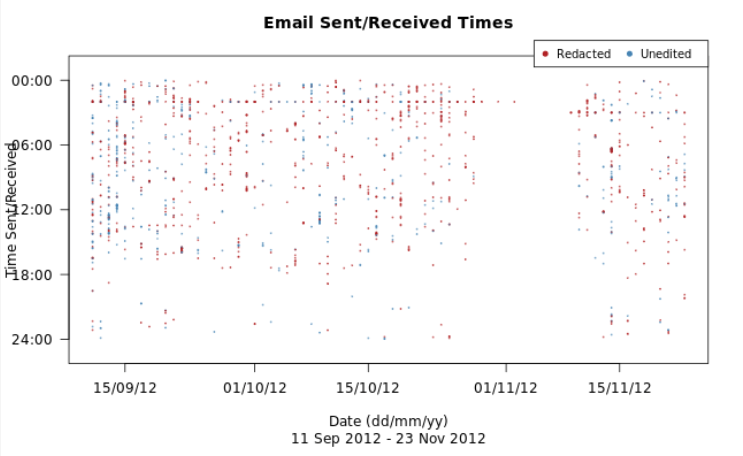
\includegraphics[height=0.22\textheight]{EmailSentRecdSept11toNov23} &
  \includegraphics[height=0.22\textheight]{InnerCircleSept11ToNov23} \\
  &\\
  {\small (a) An empty email block: October 30 - November 9} & {\small (b) Inner Circle: Correspondent info by colour; volume by thickness.}
  \end{tabular}
  \caption{Metadata: Time, date, redaction, correspondents, volume, source type.  Filtered: Sept. 11 to Nov. 23, 2012.  
  }
  
	\label{fig:teaser}
}

%% Uncomment below to disable the manuscript note
%\renewcommand{\manuscriptnotetxt}{}

%% Copyright space is enabled by default as required by guidelines.
%% It is disabled by the 'review' option or via the following command:
% \nocopyrightspace

\vgtcinsertpkg

%%%%%%%%%%%%%%%%%%%%%%%%%%%%%%%%%%%%%%%%%%%%%%%%%%%%%%%%%%%%%%%%
%%%%%%%%%%%%%%%%%%%%%% START OF THE PAPER %%%%%%%%%%%%%%%%%%%%%%
%%%%%%%%%%%%%%%%%%%%%%%%%%%%%%%%%%%%%%%%%%%%%%%%%%%%%%%%%%%%%%%%%

% Commands with arguments
\newcommand*{\TODO}[1]{\textcolor{red}{TODO #1}}
% See http://tex.stackexchange.com/questions/251460/how-to-put-symbols-of-equal-size-on-top-of-each-other?noredirect=1#comment599930_251460

\begin{document}
%% the only exception to this rule is the \firstsection command
\firstsection{Introduction}
\maketitle
The 2016 U.S. Presidential election was one of the most contentious in history.  The existence and possible content of Hillary Clinton's private email server dogged former Secretary Clinton's bid for the U.S. presidency and was doubtless a contributing factor to her surprising defeat by Donald Trump.

On March 16, 2016 Wikileaks  published a searchable archive \cite{Wikileaks} containing the contents of more than 30,000 emails (and attachments) that were sent to and from Secretary Clinton on her private server.  The documents were provided as pdfs by the U.S. Department of State in response to Freedom of Information Act (FOIA) \cite{FOIA} requests.  The State Dept. also provided a searchable web archive of the documents, released in several instalments from May 2015 to March 2017\cite{StateDeptFOIA}.   Both sites provide a  useful tool for anyone searching for particular terms in these documents.  The Wikileaks site was put to much use by investigative reporters, and others, to search for topical news items.

What is critically missing from either site is a facility to learn summary, or statistical, features across all, or groups of,  emails.   A separate site where visual displays of summary features of the emails, which can be filtered by user selection, would go a long way towards filling this need.  The site would be \emph{complementary} to the more typical ``content search and record display'' site as provided by either online archive.   Add general internet search in a third browser, and the three combined would provide the means to actively explore the contents of any email archive.    One imagines, for example, having three browsers open simultaneously, one for the data base search (e.g. Wikileaks), one for statistical visualization and exploration (proposed here), and one for internet search (to provide important context for the other two services).  Each fills a need not met by the other two; the synergy of all three provide the user a powerful set of investigative tools.

In this paper, we describe an implementation of such a visual analytic service and illustrate it on the Secretary Clinton's e-mail archive.  The implementation is located at  \texttt{rshiny.math.uwaterloo.ca/clinton} where any visitor may interactively explore summary features  of the entire corpus of emails.   Different visual displays present different salient features from all selected emails; emails can be selected via a variety of interactive filters.   All displays are reactive and update simultaneously in response to user interaction with the data filters.  Together, filters and displays provide a visual analysis service that can be used to quickly learn more about, and to discover some (possibly unanticipated) patterns in, the emails. 

The paper is organized as follows.  We provide a brief timeline on the private email server to provide sufficient context for the work.  Readers more familiar with the background may wish to skip to the next three sections where the implementation is described.  Section \ref{sect:data} discusses the source of the data, its extraction and cleaning,  details of the metadata,  redaction codes as quasi-metadata,  and our limited use of the actual email content. 
Section \ref{sect:Displays} describes the displays used and illustrates them on the data. These include a spoked network plot, an email volume time series plot, a scatterplot of daily sending times, a barplot of exemption codes, and term frequency displays. Section \ref{sect:Filters} presents the interactive filters that can be applied to change the displays.  With the implementation described, some interactive analyses of the Clinton email archive are conducted to give a quick overview of the utility of the service.  We find some interesting, and potentially contentious, patterns in the email correspondence and check these against information found from Google searches for the dates in which the patterns occur.  The section closes with caveats on over interpretation of these analyses.  Some closing thoughts are given in the final section.

%\section{Background}
%\label{sect:Background}
%
%\subsection{A brief timeline on the private email server}
%\label{sect:Background:Timeline}
\section{A brief timeline on the private email server}
\label{sect:Timeline}
While the following timeline is somewhat abbreviated, it should serve to raise some of the major issues and concerns related to Clinton's private email server and its contents.  It also introduces some of the principal characters involved.  More complete and in depth timelines are readily available elsewhere (e.g. \cite{attkissonTimeline, thompsonTimeline, WashPostTimeline, clintonWikipedia, TimeMagEverything}).

On November 21, 2008, the New York Times reported that Hillary Clinton had decided to accept the position of U.S. Secretary of State.  On January 13, 2009 the internet domain name \texttt{clintonemail.com} was registered \cite{whoisClintonserver}; eight days later Senator Clinton was confirmed as Secretary of State.  

Public knowledge that a private email server was being used by Secretary Clinton and others for State Department and personal communications did not surface until March 2015 \cite{NewYorkTimes2015} during the course of a U.S. Congressional investigation \cite{BenghaziReport} of the September 11, 2012 attack by militants on U.S. compounds in Benghazi Libya.  

The State Department had difficulty fulfilling public FOIA and House Benghazi Committee requests \cite{TakingRootWashPost} for Secretary Clinton's government emails because she had exclusively used the private server for all her email.  On March 10, 2015,  Clinton told reporters that she turned over 30,490 emails to the State Department and deleted 31,830 emails deemed to be personal \cite{WashPostTimeline}.    Clinton had tasked three lawyers Cheryl Mills (Clinton's former chief of staff),  David Kendall (Clinton's personal lawyer), and Heather Samuelson (a State Department staffer during Clinton's tenure) to make the determinations as to which emails were work related and which were not \cite{emailVetting, thompsonTimeline}.   

On March 10, 2015 the House Benghazi Committee requested that the private email server be turned over to a neutral third party to determine which emails are personal and which are government records \cite{serverRequest}, but was informed March 27 by David Kendall that no emails remained on the private server for any kind of review \cite{serverScrubbedLawyer}.
Between March 25 and 31, 2015, Paul Combetta (then the server's system administrator), erased all backup copies using \texttt{BleachBit} (see \texttt{www.bleachbit.org}).    

Combetta, Mills, and Samuelson were later granted partial immunity by the Justice Department during the FBI investigations into the private email server, as were two others: Bryan Pagliano (original server manager) and  John Bentel (former director of Information Resources Management for the State Department's Executive Secretariat) \cite{immunityPolitico, immunityDailyCaller, immunityIT}.  

On April 12, 2015 Clinton announced that she would be running for the U.S. Presidency.  On July 24, 2015, inspectors general for the State Department  and the national intelligence agencies announced that they had found classified information in the emails and that the information would have been considered classified at the time it was sent \cite{serverClassified}.  The Clinton presidential campaign declared that the emails must have been classified after the fact. On August 19, 2015, Clinton described the allegation of her mishandling classified information as simply a ``disagreement between agencies'' \cite{clintonDenialGuardian}.

Nearly one year later, July 5, 2016,  FBI Director James Comey recommended that no charges be laid against Clinton for her use of a private email server \cite{nochargeFBI}.  On October 28, 2016, Comey revealed that, in a separate investigation into former Congressman Anthony Weiner, emails belonging to his wife Huma Abedin had been found on his laptop.  Since Abedin was a close aid to former Secretary Clinton, FBI investigations were reopened into the private server usage but closed again by Comey on November 6, 2016 without charges being laid \cite{nochargeFBINov}.  In the first case Comey and the FBI were criticized by republican pundits and in the second case by democratic pundits. 

\section{The data}
\label{sect:data}
As of March 3, 2017, a total of 32,795 available emails, either to or from Hillary Clinton, have been made publicly available in pdf form as a searchable database \cite{StateDeptFOIA}.  Many of these have been redacted according to the Freedom of Information Act (FOIA) exemption codes \cite{FOIA}.  

Wikileaks \cite{Wikileaks} has provided the same redacted pdfs and, more usefully for analysis purposes, an HTML version of each pdf.  Consequently, we have used the Wikileaks database as our data source.   All data extraction, cleaning, analysis, and presentation is done using the open source statistical programming language \texttt{R}~\cite{Rsystem}.

\subsection{Data extraction and cleaning}
\label{sect:data:extrclean}
The raw HTML of each message was programmatically downloaded from the Wikileaks archive using \texttt{R} packages  \texttt{RCurl}~\cite{RCurl2016package} and \texttt{XML}~\cite{XML2016package}.  This took several hours and required the use of manually inserted system pauses to prevent time-outs in the connection, most likely due to Wikileaks DDoS (distributed denial of service) protection software. Besides avoiding such DDoS protection, these pauses are considered web-scraping etiquette and best practice.
Once downloaded, the HTML data were processed using the \texttt{R} packages \texttt{tm}~\cite{tm2008paper, tm2017package}, \texttt{stringr}~\cite{stringr2016package}, and \texttt{SnowballC}~\cite{snowballc2014package}.   

After downloading the raw HTML and extracting the data of interest, the resulting data was stored in \texttt{csv} files to provide the flexibility to load the data into any architecture or analysis tool desired.  These will be transferred to a relational data base should our server traffic warrant it.

\subsection{Metadata}
\label{sect:data:metadata}
From the HTML of each email we extract as best we can the identity of the persons sending and receiving the email as well as the date and time at which the email was processed by the server. The fields used were the address to, address from, contact name to, contact name from, subject line, and time. As well, forwarding chains of email addresses were captured through the identification of any to or from fields followed by emails within the text. In cases where no contact name was present the address was substituted. When the address was missing no imputation was completed. Carbon copy information was not extracted.

The HTML was constructed from email printed out, redacted, and then provided as pdfs by the State Department.  Consequently, detailed email header information as would normally be available electronically is mostly missing.   All time stamps appear to be the local date and time at which the server sent or received that email (e.g. no time zone or other source time or IP chain information is available).  Moreover, because of redaction (typically FOIA exemption B6 ~\cite{FOIA}),  sender and receiver emails may have truncated domains,  contain only the person's name, or be missing altogether.  In cases where both \texttt{From} and \texttt{To} are entirely missing we do not impute values  (e.g. see \texttt{https://wikileaks.org/clinton-emails/emailid/31599}).

Using regular expressions to extract the metadata was occasionally challenging and it is always possible that some fringe cases have been mishandled.  On the whole the metadata is fairly consistent and only rarely do some impure and messy addresses and contact names arise  due to irregular spacing or placement of text within the HTML code.  One such fringe case is Huma Abedin's \texttt{clintonemail.com} email account which will show in the displays as an overly long string.  We have chosen not to special case this but leave it as is.

Where possible, the email addresses have also been parsed so that they may be classified into one of four categories: those which are \texttt{.gov},  those which are \texttt{.mil},  those which are identifiable as coming from a domain that is neither  \texttt{.gov} nor  \texttt{.mil}, and those whose domain was not identifiable from the data.
\subsection{Redaction information}
\label{sect:data:redact}
Emails that are redacted are marked as such by the string ``RELEASE IN PART'' and by the presence of one or more of nine FOIA exemption codes B1, B2, \ldots, B9  marking the place where text is missing (redacted).  This provides two further pieces of quasi-metadata (since it is not actual email content) that can be used in analysis.
\subsection{Content information}
\label{sect:data:contentinfo}
The entire (redacted) content of each email is available on the State Department and Wikileaks sites and the user is encouraged to view it there (the pdf forms are more informative, especially in appreciating the extent of the redactions).  To provide some coarse statistical summaries of the content, all word tokens are extracted and partially processed to reduce their number.  For example,  ``stopwords'', as identified by the \texttt{stopwords} function (with both  \texttt{kind = "en"} and  \texttt{kind = "SMART"}), or as from a set of custom stopwords, were removed.  Remaining words were stemmed by the \texttt{stemDocument} function from \texttt{tm} and \texttt{SnowballC}.   While neither the stopword lists nor the stemming tools are particularly well tuned to this corpus of emails, they nevertheless provide some hints about the topics covered.  

\section{Displays}
\label{sect:Displays}
\subsection{Inner circle}
\label{sect:Displays:circle} 
This display takes the most frequent correspondents (max. 20) in the selected emails and arranges their email addresses  at the ends of  equiangular spokes having Secretary Clinton as hub.  The hub is coloured red to show that this account is known not to be a government sponsored account (either \texttt{.gov} of \texttt{.mil}).  Every account that is identifiably not a government sponsored account is coloured red.  Those that are identifiably government are coloured either blue (for \texttt{.gov}) or black (for \texttt{.mil}, if any appear).  Those which can not be determined as either government or not, are coloured orange.

\begin{figure}[h]
\begin{center}
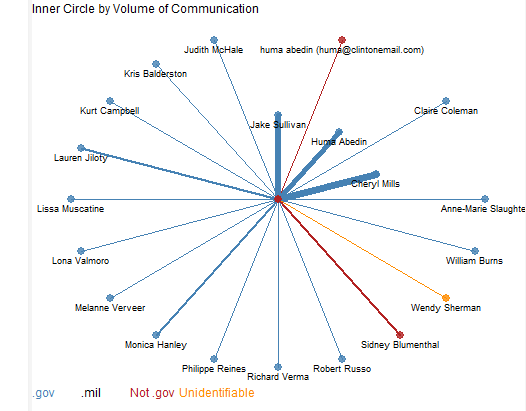
\includegraphics[width=0.95\linewidth]{SpiralNetworkFullTime}
\caption{Inner Circle over all correspondence}
\label{fig:InnerCircleAll}
\end{center}
\end{figure}
Figure~\ref{fig:InnerCircleAll} shows the top 20 correspondents (or ``Inner Circle'')  over all emails in the collection.
Note that Huma Abedin appears both as a blue  \texttt{.gov} account and as a red non-government (\texttt{clintonemail.com}) account.   The other red account is that of Sidney Blumenthal.  This has been a source of some controversy  \cite{BlumenthalControversy, NYTBlumenthalBenghazi}, since he had been rejected by the State Department yet appears to have provided Secretary Clinton advice throughout her tenure.  Wendy Sherman appears as orange. Sherman was appointed by Clinton to be Under Secretary of State for Political Affairs in 2011 and the high frequency of Sherman emails dates from this time.  Nevertheless, from this archive the email address could not be identified definitively as being either government or non-government.  Either the address was redacted for privacy reasons (a B6 FOIA exemption), or it was simply unavailable in the header provided by the WikiLeaks HTML \cite{WikileaksPull} (e.g. occasionally, a blank header appeared in the WikiLeaks HTML that was not present in the pdf; we did not correct for these manually).

The width of each spoke is proportional to the volume of emails between correspondents.  Whenever the difference in volume is great enough,  correspondents are separated into two groups: those with the greatest correspondence have shorter spokes visually placing them ``closer'' to Clinton.  As Figure~\ref{fig:InnerCircleAll} shows shows, Clinton's closest inner circle are her closest aides Huma Abedin, Cheryl Mills, and Jake Sullivan.
\subsection{Email volume}
\label{sect:Displays:volume}
Figure~\ref{fig:VolumeAll} 
\begin{figure}[h]
\begin{center}
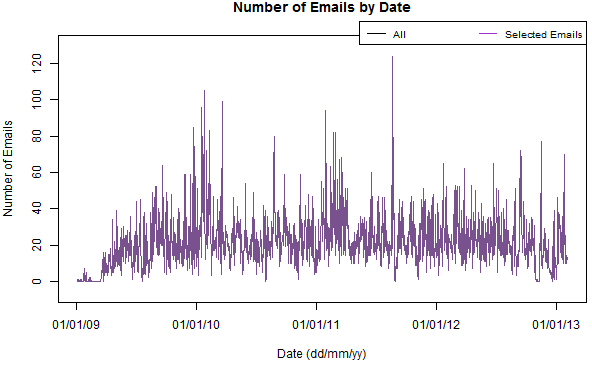
\includegraphics[width=0.95\linewidth]{VolumeFullTime}
\caption{Email Volume: All emails (top) ; Those sent by Clinton (bottom)}
\label{fig:VolumeAll}
\end{center}
\end{figure}
presents two time series showing the volume of emails for each day.  In grey at top is the daily total; in magenta at bottom is the total for the subset selected by the filters.  In Figure~\ref{fig:VolumeAll}, the bottom series is the total daily emails that were sent \emph{from} Clinton.

Over the four year scale shown in Figure~\ref{fig:VolumeAll}, the display is quite busy.  Even so, a few features stand out.  For example, there is a notable lack of email from the first few months of Clinton's tenure;  there is essentially no email from Clinton at the beginning and very little to her.   

One also notices the spikes of email activity.  These can be checked against world events to generate hypotheses about what might be occurring to cause such spikes.  For example, the largest spike occurs on August 21, 2011, the beginning day of the battle for Tripoli and on which it was reported that two of Qaddafi's sons had been captured \cite{battleTripoli}.  It is also the day on which the famous ``tick tock Libya'' email is composed by Jake Sullivan providing a timeline crediting Secretary Clinton with leading the U.S.  policy on Libya ``from start to finish'' \cite{tickTockLibya}.  Much of the email that day is redacted (B5 primarily).   Other peaks (and valleys) of activity could be similarly investigated.

\subsection{Email times}
\label{sect:Displays:times}
Figure~\ref{fig:TimesAll}  
\begin{figure}[h]
\begin{center}
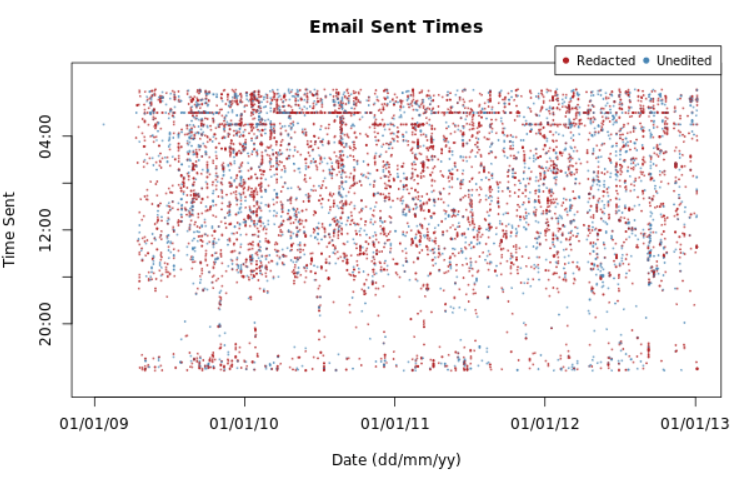
\includegraphics[width=0.95\linewidth]{DailyFullTimeFromClinton}
\caption{Email time patterns: all emails sent from Clinton}
\label{fig:TimesAll}
\end{center}
\end{figure}
shows all emails sent by Clinton over the four year period.  Each email appears as a point determined by the time that it was sent.  The calendar date determines the position on the horizontal axis,  the (24hr) time of day determines the vertical.   Points are coloured red if any part of that email was redacted, and blue if it was released in full.   Alpha blending is used to minimize the effect of over-plotting.
 
A few patterns are easily discerned.  For example, the least amount of email appears for a few hours around  20:00 hours, or 8 PM.  Evenings appear to be when email traffic is lightest.  Otherwise, for the most part, it seems fairly uniformly distributed throughout.  Midnight is at the top (and bottom) of the plot, so it would seem that email will occur mainly from midnight until about 4 or 5 PM.   

If these are the actual times Secretary Clinton composed and sent email, it suggests that much of that activity occurred in the middle of the night.  We might alternatively choose the low email activity period to mark the actual ``downtime'' between ``days'' (now interpreted as low-activity separated 24 hour email cycles);   to this end, it is possible to select 6 PM as the ``end'' of a 24 hour email cycle rather than midnight.   Though it better represents the rhythm of correspondence, this definition of the daily email cycle is unnatural to most people and so could be confusing to some users (hence by default the break occurs at midnight). 

Note also the surprisingly regular horizontal lines that appear across the top of the plot.  This regularity is suggestive of some automated schedule for the server which causes the email to stack up before being recorded at either 2 or 3 AM.  The switch between these two times matches exactly the dates where daylight savings time switches in North America.  

When the received emails are added to the plot, the pattern is essentially the same (though much denser) and the horizontal lines where the server has scheduled something are even clearer.

\subsection{FOIA exemptions}
\label{sect:Displays:FOIA}
U.S. Freedom of Information Act (FOIA) exemption codes B1 through B9 are used anywhere in an email where information has been redacted.  For the authoritative definition of the codes the act itself should be consulted \cite{FOIA}.  Briefly, a redaction is marked as B1 for national security and foreign policy matters,  B2 for personnel practices, B3 for statutory exemptions,  B4 for trade secrets or financial information obtained in confidence,  B5 for inter- or intra-agency memoranda,  B6 for personal privacy,  B7 for records compiled for law enforcement,  B8 for records prepared in relation to financial monitoring institutions, and B9 for geophysical and geological information concerning oil and gas wells.   Each email can contain redactions for any number of exemption codes.

Figure \ref{fig:FOIAcodes}
\begin{figure}[h]
\begin{center}
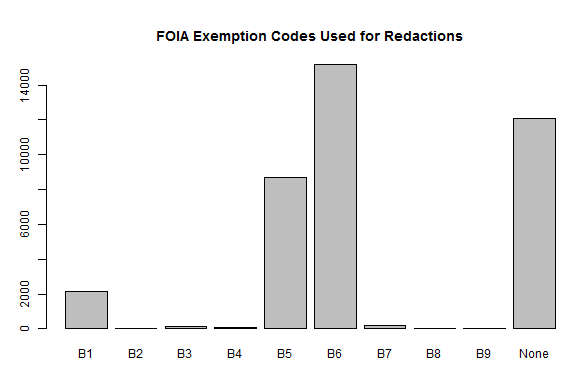
\includegraphics[width=0.95\linewidth]{ExemptionsFullTime}
\caption{FOIA barplot: Exemption codes from all email}
\label{fig:FOIAcodes}
\end{center}
\end{figure}
is a barplot of all FOIA exemption codes found in all of the emails.  As can be seen, B1 redactions made for national security and foreign policy reasons account for a small portion of all redactions made,  though this amounts to more than 2,000 emails in the collection.   Nearly half of the emails contain B6 exemptions, those made to protect personal privacy.   The inter-agency, intra-agency exemption B5 is used in more than 8,000 emails.  This code has come under some criticism from advocates for transparent government as being overly applied \cite{unredactedB5}.  The remaining codes appear in very few emails and about 12,000 emails, or about a third of them, are not redacted at all.

As with all other displays, the FOIA barplot will update in reaction to all filters and so provides a useful tool to identify co-occurrence of codes over any selection of emails.  Conversely, filtering on FOIA codes can be interesting to see who is privy to correspondence of varying sensitivities, especially B1 and B5.

\subsection{Term frequency and TFIDF}
\label{sect:Displays:TFIDF}
The 20 terms (stemmed words excluding stopwords) which appear in the greatest number of the emails selected are displayed as those having ``Highest Frequency''.  
\begin{figure}[h]
\begin{center}
\begin{tabular}{ccc}
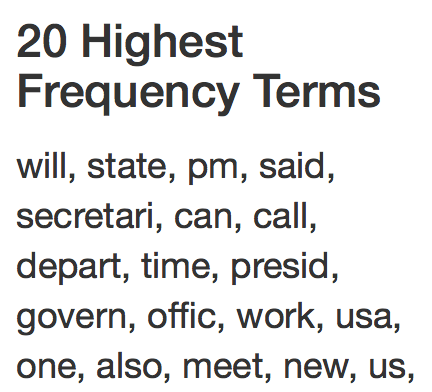
\includegraphics[width=0.4\linewidth]{HighFreqAll} &
$~~~~$ &
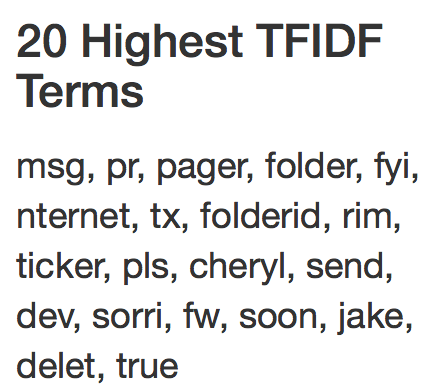
\includegraphics[width=0.4\linewidth]{HighTFIDFAll} 
\end{tabular}
\caption{Top 20 terms appearing in all emails}
\label{fig:top20all}
\end{center}
\end{figure}
Those terms which appear frequently within some emails but less frequently across emails will have a high tf-idf (term frequency - inverse document frequency) score.  The top 20 scoring of these in the selected emails are shown in the ``TFIDF'' display. 
The top 20 shown in Figure~\ref{fig:top20all} are for all emails in the corpus; these will change depending on the filtering.

The terms give some limited insight into the contents of the email.  As seen in Figure~\ref{fig:top20all}, for example, the first names of two of Clinton's closest aides, Jake Sullivan and Cheryl Mills,  appear under TFIDF but not  as high frequency terms.  One problem with tf-idf for this e-mail corpus is that many emails contain email chains which grow as each person replies; this could magnify the within email frequency for some terms.

As mentioned in Section~\ref{sect:data:contentinfo}, the stemming and stopword removal provided by the package \texttt{tm} in \texttt{R} is challenged by this messy and non-standard data. The list of stopwords had to be supplemented so as to avoid uninformative action verbs such as 'will' and 'can'. The stemming algorithm was also challenged by typographical errors in emails and the proliferation of acronyms (e.g. for individuals and government abbreviations).   

\section{Filters}
\label{sect:Filters}
There are only three filters but each one affects all data displays.  As each filter is changed, every display redraws itself on the filtered data, immediately in reaction to the change.  In this way, the filters can be used together to focus on particular subsets of the emails or simply to observe how the display patterns change with the filter being applied.
\subsection{Time filtering}
A sliding time window 
\begin{figure}[h]
\begin{center}
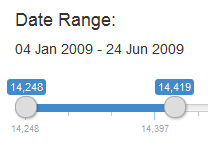
\includegraphics[width=0.35\linewidth]{DateSliderImage}
\caption{Time slider: move either end, or move the interval}
\end{center}
\label{fig:timeSlider}
\end{figure}
filters the emails displayed to those whose date lies between the two end points.
The size of the time window is changed by  moving either end, either by mouse click and drag or by selecting an end to move with the arrow keys. The whole time window is moved by selecting the middle bar and either dragging it or moving it with the arrow keys.

This filter is simple but powerful.  All emails are displayed when the range covers all dates.  Moving the end points towards one another allows the user to focus the displays on any particular range, down to as fine as all emails on a single day.  With a fixed range of days, for example a two week period,  dragging the middle bar from left to right will have each display smoothly update over time.
%
%Time filtering within the app can be completed at the level of individual days. The use of the mouse to click and drag the slider boundaries allows for large, rapid changes in the date range specified, while clicking on one of the boundaries and using the arrow keys allows for fine selection of the date range via single days. As well, clicking and dragging the blue bar in between the boundaries allows the user to sweep the data with an interval of a fixed width. Clicking the middle bar and using the arrow keys allows the user to shift the range selected by individual days, analogously to the boundaries.
\subsection{Sent or received}
A drop down menu 
\begin{figure}[h]
\begin{center}
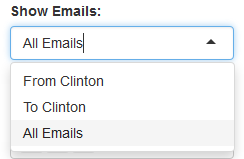
\includegraphics[width=0.35\linewidth]{ToFromImage}
\caption{Filtering on whether Clinton sent or received the email, or either}
\label{fig:toFromFilter}
\end{center}
\end{figure}
is used to select those emails which Clinton sent, or received, or either (i.e. sent or received).  The default is ``All Emails'', which is the same as no filter being applied for sent or received.  Choosing ``From Clinton'' selects for display only those mails sent by Secretary Clinton, choosing ``To  Clinton'' selects only those emails which she received.  This might be used, for example, to explore whether the inner circle of correspondents changes depending on whether Secretary Clinton is emailing them, or they are emailing her.

Note that if neither the ``From:''  nor ``To:''  were captured from the HTML, then such emails can appear only when ``All Emails'' is selected.


\subsection{FOIA exemptions}
Multiple filtering by FOIA exemption codes is supported using a box selection area. 
\begin{figure}[h]
\begin{center}
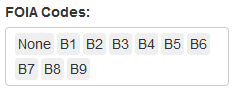
\includegraphics[width=0.55\linewidth]{FOIABoxImage}
\caption{FOIA codes:  Emails containing any of these codes appear}
\label{fig:selectFOIA}
\end{center}
\end{figure}
Figure~\ref{fig:selectFOIA} displays the codes that are selected for email display.  Any email having one or more of these codes will appear in the displays.  To not have emails display with a B1 exemption code, for example, then the user selects and deletes the B1 from the list (multiple selection is enabled).  Or to have only the emails which  contain B1 redactions displayed, all other codes can deleted from the list.  

Codes are returned to active display at any time by clicking in the display box and selecting them again from a drop down menu of the excluded codes.  Any number of codes  (one or more) can be selected to be included in the displays.

\subsection{Auxiliary information}
To demonstrate how other sources of information can easily be used to supplement the metadata found in the email archive, we consulted the State Department website and retrieved Secretary Clinton's official foreign travel schedule  \cite{ForeignSched}.  This information was added to the display as a simple check box ``Display Foreign Travel Schedule''.  When checked, light blue vertical bars appear on the  email volume time series display.  Appearing behind the series, these mark time periods when Secretary Clinton was travelling outside the U.S. on State Department business according to the published schedule.

\section{Some interactive analyses}
\label{sect:Analysis}
Each of the displays and filters described in the previous sections gives a slightly different informative view of summary features of the email archive.  Their analytic power is considerably amplified when used together.  

Rather complex queries can be formed involving date, classification code, and whether Clinton is sending or receiving email.  Moreover, given a particular pattern in one display, its relation to that in another can be of considerable interest.   Together with access to the archive contents and an internet search engine, an enormous amount can be learned from these visual analytic tools.

In this section, we explore a few avenues of enquiry that might naturally arise.  At best these only hint at the analytic power that interactive filtering and display can bring to bear on an email archive.  The user is encouraged to try it themselves at \texttt{rshiny.math.uwaterloo.ca/clinton}to get a fuller appreciation of the power of the tool.  Those who are exploring the corpus will find it useful for generating hypotheses that might be tested against other sources.   This is the approach taken here.  Conversely, those more knowledgeable about the contexts surrounding Secretary Clinton and her private email server might use the visual analytic tool more as a means to test hypotheses already held.

\subsection{The last two years}
We begin our interactive analysis by looking at  email patterns in the last two years of Clinton's tenure as Secretary of State.  

Figure~\ref{fig:lastTwoYears} 
\begin{figure}[h]
\begin{center}
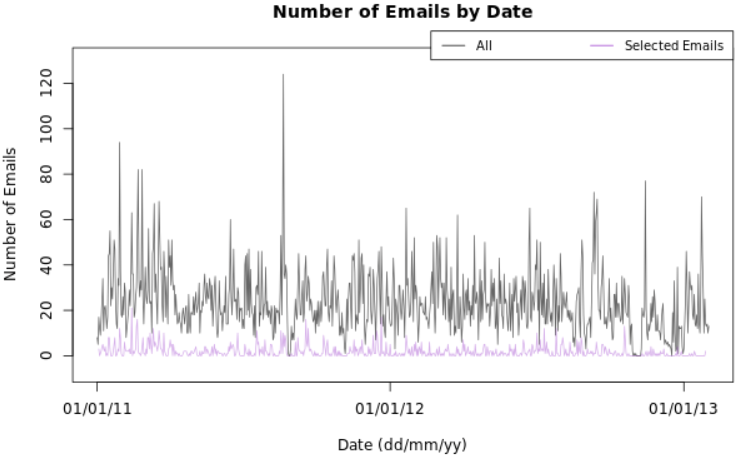
\includegraphics[width=0.95\linewidth]{EmailVolumeB1LastTwoYears}
\caption{Last two years:  Selected Emails are those that are B1 redacted}
\label{fig:lastTwoYears}
\end{center}
\end{figure}
shows the email volume time series over this period. 
This is accomplished by simply having the right end of the time slider of Figure~\ref{fig:timeSlider} as far right as possible and then moving the left most end towards the middle of the time period until January 1, 2011 is reached.   Note, however, that in addition to filtering on time we have chosen to also filter on FOIA exemption code, selecting only those emails containing one or more B1 (national security and foreign policy matters) redactions.  The magenta time series at the bottom then shows all emails, sent or received by Clinton, in the last two years of her tenure which were redacted in part by the State Department (after the fact, not at the time) as being B1 FOIA exempt.  As can be seen, there are \emph{relatively} few of these.

Recall from Section~\ref{sect:Displays:circle} that the tallest spike of Figure~\ref{fig:lastTwoYears} corresponds to the beginning of the battle for Tripoli (August 21, 2011).   The next largest spikes appear at the far left of this time window, at the beginning of 2011.  We might choose to compress the time window more, to focus on the early 2011 section of the emails.  Bringing the right end of the time slider in to April 15, 2011 produces the series of Figure~\ref{fig:early2011B1}.
\begin{figure}[h]
\begin{center}
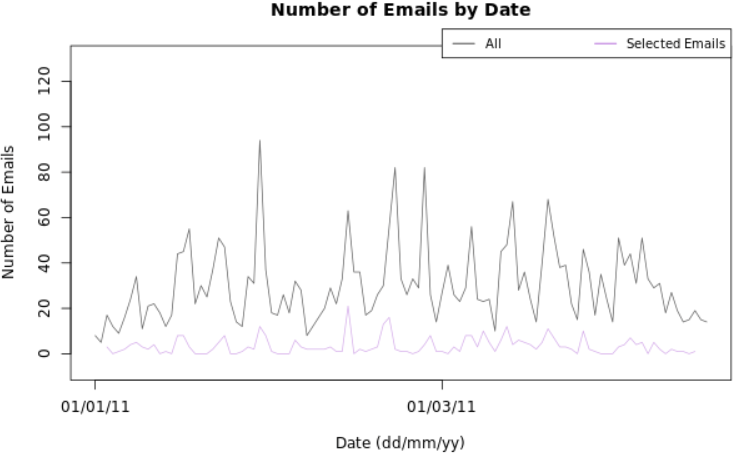
\includegraphics[width=0.95\linewidth]{EmailVolumeB1JanApril2011}
\caption{Jan. 1 -- Apr 15, 2011:  Selected Emails are those that are B1 redacted}
\label{fig:early2011B1}
\end{center}
\end{figure}

As can be seen, there continue to be highs and lows of email activity.   The highest peak now is at the left, though closer to the centre of Figure~\ref{fig:early2011B1} than it had been in Figure~\ref{fig:lastTwoYears} .  This is January 29, 2011, the day after President Mubarak of Egypt has ordered the army into the streets of Cairo to quell protests \cite{cairoTanks2011, cairoResponse2011}.  Dipping into the contents of the Wikileaks email archive, much of the email on this day is seen to be about managing this Egyptian crisis.  

Just to the right of this peak, there are several more.   At this time, international forces are gathering to consider Libya and its leader Muammar Gaddafi.  Consulting Jake Sullivan's ``tick tock on Libya'' timeline describing Secretary Clinton's leadership on the Libyan crisis, we move the sliders in again, this time to focus on the time range from February 25 (when Secretary Clinton announced the suspension of the Libyan embassy in Washington) to March 18 (the day after Secretary Clinton had secured ``\ldots Russian abstention and Portuguese and African support for UNSC 1973, ensuring that  it passes. 1973 authorizes a no-fly zone over Libya and `all necessary measures' - code for military action - to protect civilians against Gaddafi's army \ldots'' \cite{tickTockLibya}).  On March 19, 2011 NATO military operations in Libya began \cite{LibyaTimelineWiki}.

The readjusted time series are shown in Figure~\ref{fig:EmailVolumeB1LibyaBuildup}.
\begin{figure}[h]
\begin{center}
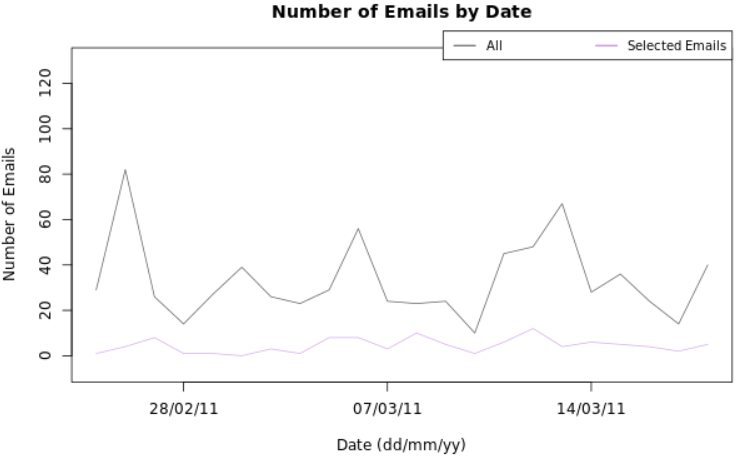
\includegraphics[width=0.95\linewidth]{EmailVolumeB1LibyaBuildup}
\caption{Feb. 25 -- March 15, 2011:  Selected Emails are those that are B1 redacted}
\label{fig:EmailVolumeB1LibyaBuildup}
\end{center}
\end{figure}
The left most spike in Figure~\ref{fig:EmailVolumeB1LibyaBuildup}  is the rightmost spike of the pair of approximately 80 emails from Figure~\ref{fig:early2011B1}.   
Of course all other displays have been updating every time the time slider is adjusted.  

Some sense of the content of the emails can be had from the updated term frequency displays shown in Figure~\ref{fig:TermFreqB1LibyaBuildup}.
\begin{figure}[h]
\begin{center}
\begin{tabular}{ccc}
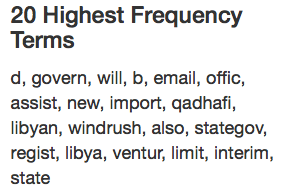
\includegraphics[width=0.4\linewidth]{TFIDFB1LibyaBuildup} &
$~~~~$ &
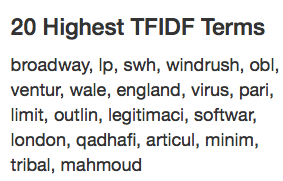
\includegraphics[width=0.4\linewidth]{TermFreqB1LibyaBuildup} 
\end{tabular}
\caption{Frequent terms: B1 only emails, Feb. 25 -- March 18, 2011}
\label{fig:TermFreqB1LibyaBuildup}
\end{center}
\end{figure}
Not surprisingly,  Libya and its leader figure prominently in this restricted set of emails.  

Perhaps more surprising is a term like ``windrush''.  A little investigation shows that this is a reference to ``Windrush Ventures'' (e.g. see  \cite{windrushTelegraph, windrushGuardian}),  a company owned by former U.K. Prime Minister Tony Blair .  ``Windrush'' appears at the end of emails as part of Mr. Blair's electronic signature.   Mr. Blair is part of this B1 selected correspondence.

Other restrictions, as measured by the FOIA exemption codes, can be seen in Figure~\ref{fig:FOIAB12011LibyaBuildup}.
\begin{figure}[h]
\begin{center}
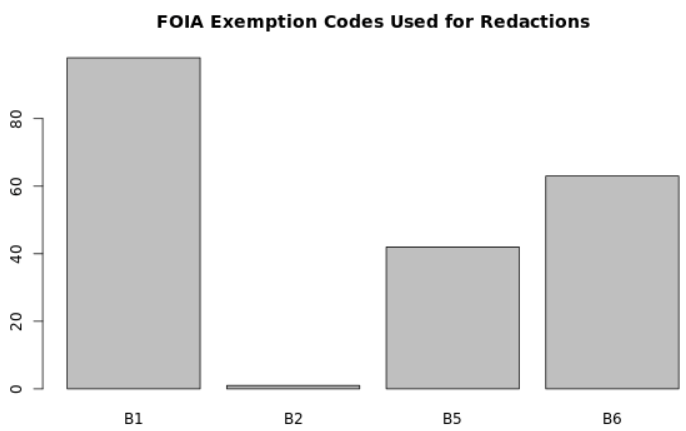
\includegraphics[width=0.95\linewidth]{FOIAB12011LibyaBuildup}
\caption{FOIA code distribution: All  B1 redacted, Feb. 25 -- March 18, 2011}
\label{fig:FOIAB12011LibyaBuildup}
\end{center}
\end{figure}
There appear to be about 100 emails in the selected set.  In addition to having B1 redactions, many of them also have B5 (inter- or intra-agency) and B6 (personal) redactions.

We might now consider the composition of the inner circle for this set of emails.  Figure~\ref{fig:InnerCircle2011B1LibyaBuildup} 
\begin{figure}[h]
\begin{center}
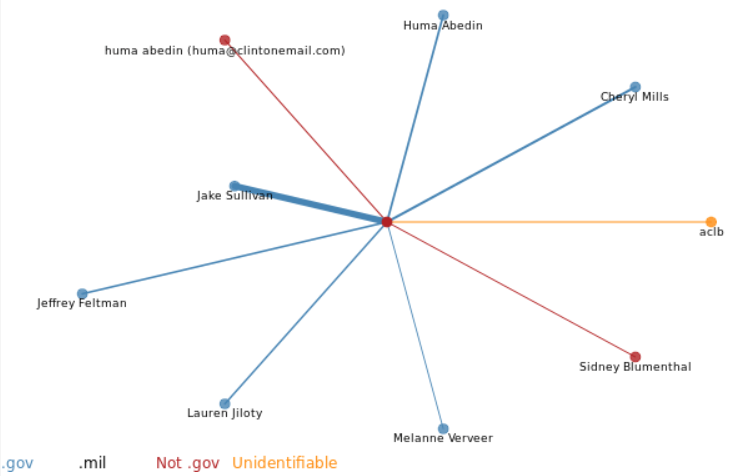
\includegraphics[width=0.95\linewidth]{InnerCircle2011B1LibyaBuildup}
\caption{Inner Circle: All  B1 redacted, Jan. 1 -- Apr 15, 2011}
\label{fig:InnerCircle2011B1LibyaBuildup}
\end{center}
\end{figure}
shows the set of correspondents.  Not surprisingly, Jake Sullivan is the principal correspondent.  Huma Abedin is next, though she is using two emails, one a government account the other a personal \texttt{clintonemail.com} account.   Sidney Blumenthal, a non-government employee, is in this inner circle of B1 exempted emails.  So too is former U.K. Prime Minister Tony Blair; this is the unidentifiable domain account \texttt{aclb}.
It should be noted that there could be other accounts which do not appear in the inner circle because their emails were not present in the email record.  See Section~\ref{sect:data:metadata}.

We could continue to drill down into this information, checking the (unredacted) contents of the emails themselves from either the Wikileaks or State Department sources.  We might also more closely connect email dates and correspondents with world events.   Instead, we now turn our attention to another feature which appears in Figure~\ref{fig:lastTwoYears}.

\subsection{An email gap?}
\label{sect:emailGap}
Towards the very right of Figure~\ref{fig:lastTwoYears} there appears to be an anomaly in both time series.  There is a noticeable flat area at zero in both series.  If we move the leftmost time sliders to the June 1, 2012, and the rightmost to the end, February 1, 2013, we have the email volumes for the last 8 months of the archive.  The resulting series are shown in Figure~\ref{fig:EmailVolumeB1Jun1On}.
\begin{figure}[h]
\begin{center}
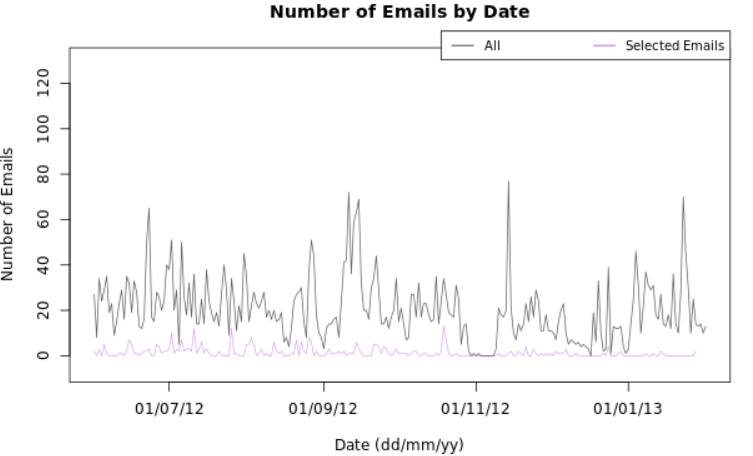
\includegraphics[width=0.95\linewidth]{EmailVolumeB1Jun1On}
\caption{June 1, 2012 -- February 1, 2013:  Selected Emails are those that are B1 redacted}
\label{fig:EmailVolumeB1Jun1On}
\end{center}
\end{figure}
There appears to be no emails for a fairly large chunk of time.  In fact, there are few or no emails in the archive from October 30 to November 9, 2012.  This seems curious, given that the archive is supposed to be complete in Secretary Clinton's work-related email during this time period.  
The block of no email appears as an even more unusual pattern in Figure~\ref{fig:teaser}(a).  There the block is conspicuous by the absence amongst the emails from September 11 to November 23, 2012.  The email on which the displays of Figure~\ref{fig:teaser} are based, is no longer filtered by FOIA code.  It contains all email in the archive in this time period.  Direct examination of the archives at Wikileaks and the State Department show no mail in this empty block beyond that seen in Figure~\ref{fig:teaser}(a).

The inner circle for all emails from September 11 to November 23, 2012 is shown in Figure~\ref{fig:teaser}(b).  Those closest to Clinton in terms of volume of correspondence are Clinton aides Jake Sullivan, Cheryl Mills, and Monica Hanley.  Monica Hanley also appears with an account whose identity as government or not could not be determined.  Tony Blair and Sidney Blumenthal both appear in the inner circle, as does Wendy Sherman (though the account could not be identified as government or not).  Oscar Flores is an assistant to the Clintons, often working at their home.  The rest are identified as corresponding through government accounts.

One might ask what is happening around this time period?  In a word, Benghazi.  Five days after the assault, the U.S. Ambassador to the United Nations, Susan Rice, made a series of television appearances explaining that the attack on the U.S. Benghazi mission was a spontaneous response a  ``hateful video''  which had hours earlier caused violent protests in Cairo against the U.S. Embassy \cite{faceTheNationSept16}.   Four years later, it will be revealed as part of the House Select Committee on Benghazi report \cite{BenghaziReport} that Secretary Clinton had as early as September 12, 2012, communicated to Egyptian Prime Minister Kandil that the attack was known to be planned by Al Qaeda affiliates, it was not a protest, and that it had nothing to do with the film \cite{ClintonAdmitsAttackSept12}.  By the end of September the U.S. administration was calling it a terrorist attack \cite{factCheckerBenghazi}.  A month after the attack the administration was defending itself against charges that it deliberately downplayed a terrorist attack in Libya for political reasons in a presidential election year \cite{susanRiceWashPost2012}.   In October, focus shifted to the security at Benghazi and whether it had been reduced prior to the attack  \cite{cbsSecurity}.  The House Committee on Oversight \& Government Reform began looking into the security aspect \cite{cbsNewsHouseOversight2012} in earnest and found evidence that security issues were known and that requests from the U.S. Embassy in Libya for additional security personnel had been turned down by the State Department \cite{BenghaziSecurityTestimony}.  On October 26, CIA operatives who had defended the Benghazi mission against the terrorist attacks came forward with their story of what happened, on the ground.  They maintain that it was an organized attack and tell reporters that they were told to ``stand down'' \cite{standDownOrder}.  From October 26 to November 9 2012, no email appears in the archive as being sent from Secretary Clinton.

Moving the time sliders to cover either side of the email gap, October 22 to November 17, 2012, results in  the term frequency displays of Figure~\ref{fig:TermFreqOct22Nov17_2012}.
\begin{figure}[h]
\begin{center}
\begin{tabular}{ccc}
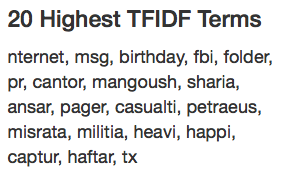
\includegraphics[width=0.4\linewidth]{TFIDFOct22Nov17_2012} &
$~~~~$ &
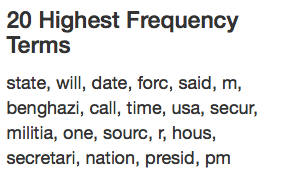
\includegraphics[width=0.4\linewidth]{TermFreqOct22Nov17_2012} 
\end{tabular}
\caption{Around the gap: All emails, Oct. 22 to Nov.17, 2012}
\label{fig:TermFreqOct22Nov17_2012}
\end{center}
\end{figure}
It would seem that emails were very much related to the unfolding political crisis of Benghazi.  Even the name of the terrorist group, Ansar al-sharia, is picked up in the tf-idf terms.

Whatever the reason for the gap seen in the archive, one thing is certain.
The story of Benghazi and its aftermath, with its piecemeal and contentious disclosures, and unfolding as it did immediately before a U.S. Presidential election, would consume much of the attention and energy of the U.S. administration, Congress, and the U.S. electorate.  It was an event that would haunt Secretary Clinton for months and years  to come \cite{benghaziTimelineWikipedia}.

\subsection{A hunt for no email}
\label{sect:emailZeros}
The discovery of the obvious email gap in November 2012 raises the possibility that there may be other, less obvious, gaps in the email archive.  

To explore this possibility,  the time slider can be adjusted to a relatively small span, say of thirty days.  This would allow gaps in email of smaller sizes to be detected.  To focus attention on Secretary Clinton's behaviour, only those emails sent from Secretary Clinton would be displayed.  
Moving the slider, from left to right, from early 2009 to early 2013, allows one to move a one month wide magnifying glass across the whole of the archive.  A few contiguous days with no email from Clinton will appear as a small horizontal line at zero in the email volume (magenta coloured and lower) time series.  Once found, the sliders can be further narrowed to identify the dates of the patch.

Following this approach, ten 
more patches can be found (in addition to that of Section~\ref{sect:emailGap}).  With the dates in hand, an internet search can be conducted to see what, if anything, might turn up to explain the patch.
%\subsubsection{You have no mail \ldots}
\subsubsection{Early days}
\label{sect:youHaveNoMail}
The first, and largest, patch occurs at the very beginning of Clinton's tenure as Secretary of State.  It is  obvious even from the full time series of Figure~\ref{fig:VolumeAll}.  Essentially no email from Secretary Clinton, and little from anyone else appears until mid to late April 2009.  

This is the time when Secretary Clinton's email habits first run afoul of the State Department as Clinton insists on using her personal Blackberry for all of her email communications.  The issue came to a head in February when National Security officials and intelligence specialists explain the risks to Cheryl Mills.  The officials were apparently not aware  of the private email server (e.g. see \cite{TakingRootWashPost}).  
%In time order, the patches and what we learned from each Google search was as follows.

\subsubsection{Three patches in 2009}
Three of the patches appear to be easily interpreted.   June 17 to June 23, 2009 coincides with Clinton's surgery for an elbow fracture after a fall \cite{ClintonFracture2009}.  A month later, from July 17 to July 23 another patch appears.  This coincides with Secretary Clinton's State visits to India and Thailand \cite{ForeignSched}.  Similarly, the absence of email from Clinton from October 11 to  October 13, 2009 corresponds to a State visit to Russia as shown in  Figure~\ref{fig:ClintonZerosOctober2009AndForeignSchedule} \cite{ForeignSched, visitRussia}.
\begin{figure}[h]
\begin{center}
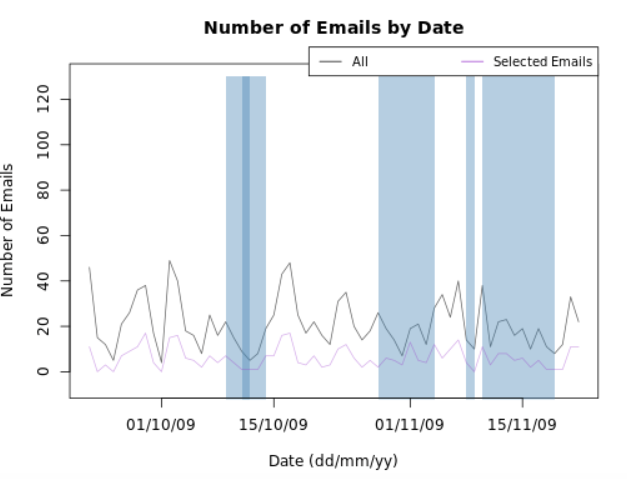
\includegraphics[width=0.95\linewidth]{ClintonZerosOctober2009AndForeignSchedule}
\caption{Oct 3 -- Oct 27, 2009:  Selected Emails are from Clinton; Scheduled foreign travel marked in blue.}
\label{fig:ClintonZerosOctober2009AndForeignSchedule}
\end{center}
\end{figure}

\subsubsection{April 11 to April 15, 2011}
%The next patch chronologically comes in 2011, from April 11 to April 15.   
On the last two days of %the 
this patch, Secretary Clinton met with other NATO Foreign Ministers in Germany \cite{ForeignSched}.   Notably, in an April 10, 2011 email, Huma Abedin forwards Clinton the ``Stevens Update'' from Timmy Davis.  The email describes Ambassador Stevens's concerns about the situation in Ajdabiyah (less than 150 km from Benghazi) where he is considering leaving Benghazi \cite{StevensUpdate}.

\subsubsection{August 27 to August 29, September 1, 2011, 2011}
%From August 27 to August 29, and again in September 1, 2011 no emails are sent from Clinton.   
No foreign travel appears on the schedule.  Notable events include ``Russian hackers'' tried to gain access to Clinton's email accounts through phishing \cite{russianHackers2}; a significant Clinton Foundation donor, Rajiv K. Fernando, was added by Cheryl Mills to the International Security Advisory Board  \cite{clintonDonorSecurity}; State Department executive secretary Stephen Mull is rebuffed by Huma Abedin when he suggests replacing Clinton's personal BlackBerry by a ``department-issued'' one \cite{earlyEmails}.

\subsubsection{End of March,  beginning of April, 2012}
%The next patch appears at the end of March, the beginning of April, 2012.  
The exact dates were March 27 and 29, the range from March 31 to April 3, and then again on April 10.   Few, but not zero, emails were sent between these dates.  Google search does not turn up much other than the fact that Clinton Staffers seem to be vetting email \cite{tightReinRecords, staffVetEmail}, and that Clinton had received an email which in part contained classified material \cite{classifiedInPart}.

\subsubsection{End of August,  beginning of September, 2012}
No emails are found sent from Secretary Clinton's email from August 27 to August 30 and September 1, 2, and 6, 2012, all just before the Benghazi attack.  Much has already been written about this time period.  Here we add that in a cable to ``SECSTATE'' dated August 8 (via Hanna Draper) and entitled ``The Guns of August: security in eastern Libya'' from Ambassador Stevens was the comment ``What we have seen are not random crimes of opportunity but rather targetted and discriminate attacks'' \cite{gunsOfAugust}.  According to the Benghazi Report,  during August the number of State Department security agents assigned to the embassy in Tripoli dropped from 34 to 6 \cite{BenghaziReport}.

\subsubsection{Two patches in December 2012}
The last two patches appear 
shortly after the email gap from Section~\ref{sect:emailGap}.  As seen in Figure~\ref{fig:ZeroEmailsDec2012}
\begin{figure}[h]
\begin{center}
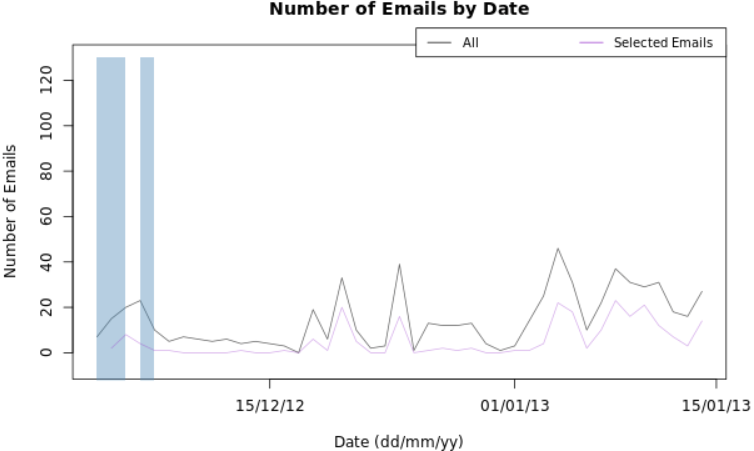
\includegraphics[width=0.95\linewidth]{ZeroEmailsDec2012}
\caption{Dec 3 -- Jan 14, 2012:  Selected Emails are from Clinton; Scheduled foreign travel marked in blue.}
\label{fig:ZeroEmailsDec2012}
\end{center}
\end{figure}
these are the two closely related gaps in December 2012 which,
% for the purposes of discourse only,  we are counting as only one of our 
%ten patches
might be counted as one large gap.
Similar to June 2009, there is an easy explanation at hand, at least for the first of these.  Clinton had suffered a concussion ``\ldots in a fall brought on by an illness'' \cite{concussion} and was recovering at home by December 15.  She had `already been forced to cancel a planned trip to the Middle East and north Africa'' \cite{concussion} that week; this is not the foreign travel shown in Figure~\ref{fig:ZeroEmailsDec2012} \cite{ForeignSched}.  

A Google search,  however, produces other news items of possible relevance.  On  December 19, four State Department employees associated with Benghazi resigned.  Three are top State officials: Eric Boswell,  the assistant secretary of state for diplomatic security;  Charlene Lamb, the deputy assistant responsible for embassy security; and Raymond Maxwell, the deputy assistant secretary for overseeing the Mahgreb nations of Libya, Algeria, Tunisia, and Morocco \cite{securityResigns, fourResign, tripoliPostResign}.  The fourth is not identified in \cite{fourResign, tripoliPostResign}.   Raymond Maxwell appears again in the news nearly two years later when, feeling scapegoated, he breaks a story to investigative reporter Sharyl Attkisson.  Maxwell alleges that in October 2012 he witnessed a Sunday afternoon document sorting session in the basement of the State Department after Congress had called for documents related to Benghazi \cite{AttkissonBenghaziBombshell, attkissonTimeline}.  Its purpose would appear to be the removal of potentially embarrassing documents.  Jake Sullivan,  Cheryl Mill, and a State Department office director ``close to Clinton's top advisors''  were said to be present (see\cite{AttkissonBenghaziBombshell}).

Also in December 2012, Cheryl Mills and Heather Samuelson were made aware of an FOIA request from ```Citizens for Responsibility and Ethics in Washington'' (or CREW) that had been filed on December 6 \cite{CREWFOIA, FOIAcall}.   The U.S. Ambassador to the U.N. Susan Rice withdraws her name from consideration as a Secretary of State to replace Clinton \cite{RiceWithdraws}.  December 2012 was a busy month.

\subsection{Caveats}
\label{sect:caveats}
As the interactive analyses above shows, there is considerable information in the metadata, especially when it can be linked to other sources of information.  However some care must be taken when conducting such an analysis.  

It is quite possible that we will only see what we want to see in the data.  The human tendency to seek out information that confirms our preconceptions has been well known since 1620 when Francis Bacon first wrote 
\begin{quotation}
``The human understanding, once it has adopted opinions, either because they were already accepted and believed, or because it likes them, draws everything else to support and agree with them.''

\noindent
Francis Bacon, \emph{Novum Organum}, Book 1, Aphorism 46 \cite{Bacon1620}

\end{quotation}
This is now called confirmation bias \cite{confBias} and it plagues much modern discussion, particularly on the internet and social media.  

By building an interactive filter and display tool for Secretary Clinton's emails we have uncovered some unusual patterns.  Many time periods show no email from Clinton.  One large period shows no mail at all.  Whether records are missing by accident or by intention cannot be determined by these tools. 
Instead, hypotheses have been generated which might be explored by others more knowledgeable.

It is particularly important to try to avoid confirmation bias when performing internet search.  For every patch where Clinton sent no email, we deliberately used a very coarse query to the Google search engine.   
Figure~\ref{fig:googleSearch}
\begin{figure}[h]
\begin{center}

\includegraphics[width=0.75\linewidth]{googleSearch}
\caption{The coarse Google search: for any patch found in March 2009}
\label{fig:googleSearch}
\end{center}
\end{figure}
shows the search query for a March 2009 patch.  We followed the same style of query for all patches that we uncovered visually.  Only the first page of hits returned from the search was examined.

As seen in Section~\ref{sect:youHaveNoMail} this was often sufficient to turn up information that explained the lack of email as naturally occurring due to injury or travel.  In other cases, the information turned up was possibly contentious and could be interpreted to suggest that the email was deliberately missing.  We do not, and cannot, suggest that this is the case.  Of course, the way in which the emails were selected to be handed over to the State Department and the subsequent erasure of all back up copies does little to dissuade anyone who might hold this view.

We were surprised to see how often something contentious showed up with the Google search for the identified patches.   To check whether such a search would nearly always turn up something contentious, we randomly selected 10 combinations of months and years over the time period of the archive (a total of 60 possible combinations).  One of the combinations we turned up matched a patch we had identified ("Dec 2012"), the remaining did not.  The complete sample (and what we found for each) was as follows:  ``June 2011''  (pro forma cable from SECSTATE that State Dept. employees change their passwords), ``Nov 2010''  (U.S. Embassy Cables appear on Wikileaks; Clinton rejects suggestion by Huma Abedin to start using  a government email account),   ``Dec 2012'' (documented in Section~ref{sect:youHaveNoMail}), ``March 2009'' (Clinton hits reset button with Russia), ``May 2011'' (Clinton delivers remarks on GlobalFood Security), ``March 2011'' (Clinton rejects talks with Gaddafi's sons; P.J. Crowley forced to resign), ``May 2012'' (State Dept. investigating computer shipments to Iran), ``Dec 2011'' (Putin accuses Clinton of encouraging Russian protests), ``June 2012'' (Geneva I conference on Syria; Bill Clinton checked with State Dept. on paid speech to group with Tehran ties; State Dept. Trafficking in Persons report), and  ``Oct 2011'' (Iranian plot to kill Saudi ambassador, State Dept. cannot confirm Gaddafi's death).   None but ``Dec 2012'' have a connection to the Benghazi controversy though two mention email.
 
 We need to also point out that the extraction of data is always an opportunity for error to occur.   For example, we have already mentioned difficulties with processing email addresses that have been partially or entirely redacted.  The Wikileaks transcription from pdf to HTML is also imperfect.  For example, the string ``b9''  appears in one email record (Doc ID: 10257) in the Wikileaks transcription\cite{errorWikileaks} as a transcription error of the day ``09'' from the original pdf.  This might be grabbed as a B9  redaction code, if one is not careful.  The same email record also has ``To'' and ``From'' header which is empty except for a date.  This header does not appear in the original pdf; rather the pdf begins with the next one inside the HTML.   There are no doubt other errors as well.  
 
 The process we have followed is an automated one.  One conducted by hand, by examining each pdf, would likely produce better data but not necessarily for more than 30,000 records.  At least a check by hand of all HTML email records with blank to and froms at the beginning could be of some value.
 
\section{Concluding Remarks}
In providing the service, we purposely focused the displays (for the most part) on simple characteristics of the emails, the so-called metadata.  There are several related reasons for this focus.  

First, metadata is often more reliable, regular, and, being easily collected, more generally available.  For Secretary Clinton's emails,  some metadata is lost, either because their source is a printed form or because it has been redacted.  Examining metadata also arguably intrudes least upon the privacy of the individual correspondents, compared at least to the email's content.  

Second, since at least the Snowden revelations (e.g. \cite{NYRsnowdenLeaks}), public discourse has grown on the potential value of metadata to those who have it.  By providing a web service where anyone can see for themselves what might be learned from metadata, we hope to contribute positively to this important discussion.  Moreover, the work-related only metadata of a public figure as senior as Secretary Clinton will hopefully resonate more strongly with other public figures  engaged in the debate (e.g.   \cite{NYRmetadata, ObamaMetadata, JebBushMetadata2015, PompeoMetadata, TrumpMetadata}) than might that of an ordinary citizen.  

Third, it is important that users realize that the value of metadata is not just in itself, where one might expect to easily discern general day-to-day habits such as one's circle of correspondents.  Rather it is that when coupled with other sources, which are abundantly and publicly available for Secretary Clinton, much more can be learned than from any one source alone.  Those who have knowledge of, or access to, other sources may filter metadata to test previously held hypotheses; conversely, exploration of metadata could uncover patterns that generated hypotheses to be tested elsewhere. 

Finally, this is a cautionary tale.  The collection and storage of metadata from any individual in our society should be of concern to all of us.  While it is possible to discern patterns from several sources, it is also far too easy to construct a false narrative, particularly one that fits an already held point of view.  As analysts, we fall prey to our cognitive biases \cite{gilgovichBook}.  Interactive filter and display of metadata from a large corpus of communications add another tool to an already powerful analytic arsenal.  As with any other powerful tool it needs to be used with caution.  

%% if specified like this the section will be committed in review mode
\acknowledgments{
This work was supported in part by
a Discovery grant from the Natural Sciences and Engineering Research Council of Canada..}

%\newpage
%$~~~$
\newpage

\bibliographystyle{abbrv}
%\bibliographystyle{abbrv-doi}
%\bibliographystyle{abbrv-doi-narrow}
%\bibliographystyle{abbrv-doi-hyperref}
%\bibliographystyle{abbrv-doi-hyperref-narrow}

\bibliography{clinton}

\end{document}
